\begin{figure*}[t]
\centering
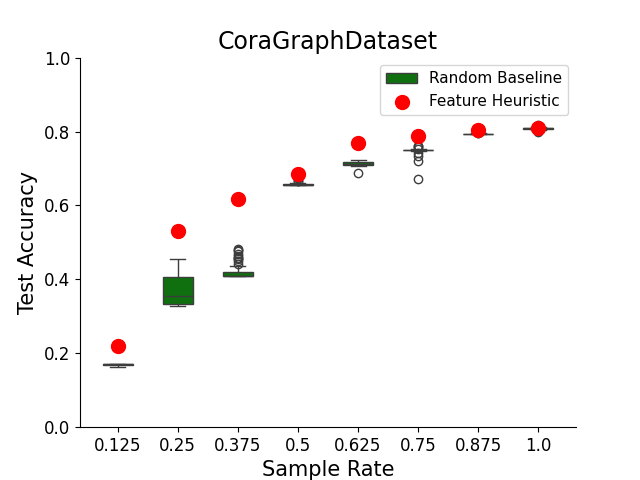
\includegraphics[width=0.32\textwidth]{img/GNN_acc_revised/CoraGraphDataset_undirected_random_baseline_boxplot.png}
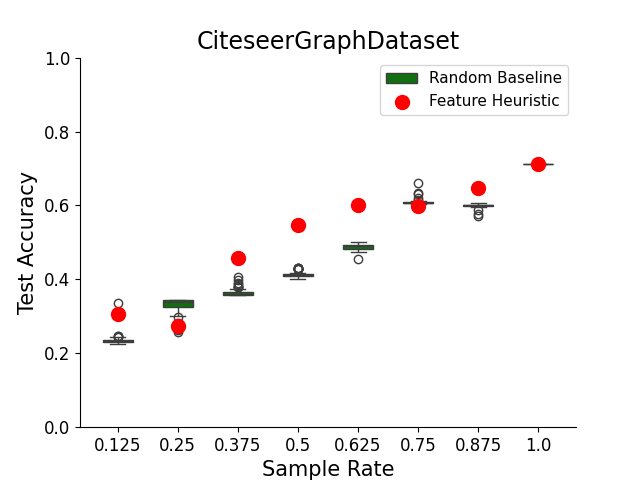
\includegraphics[width=0.32\textwidth]{img/GNN_acc_revised/CiteseerGraphDataset_undirected_random_baseline_boxplot.png}
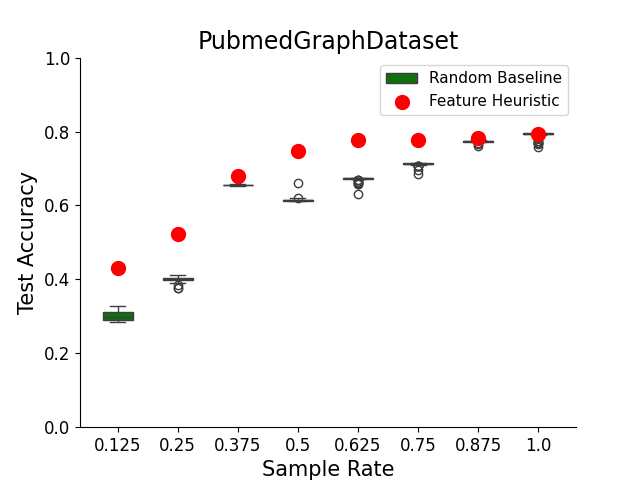
\includegraphics[width=0.32\textwidth]{img/GNN_acc_revised/PubmedGraphDataset_undirected_random_baseline_boxplot.png}
\caption{The red dots are the test accuracy of models tuned on each dataset at specific sample rates, with boxplots indicating the distribution of random baseline test accuracy. Our heuristic yields better results only except for Citeseer at 25\% of sample rate. Specifically, the differences of test accuracy are mostly recognizable at sample rates ranging from 37.5\% to 75\% across all three datasets. On average, accuracy grows slower as sample rate increases, intuitively because the marginal information is less significant with larger number of nodes already included in the subgraphs. }
\label{fig:GNN Acc}
\end{figure*}

\section{Feature homophily and homophily-based sampling}
%In this section, we present our theoretical contributions to the understanding of graph node downsampling. We firstly define feature homophily, then explain how it can be used to bound the trace of $\mathbf{L}$.

We start by introducing the notion of feature homophily, which is a requirement for our algorithm.
%and describe how graphs with moderate to high feature 
In order to make this definition compatible for graphs of different sizes, we first need to normalize $X \in \mathbb{R}^{n\times d}$ along both the feature and node dimensions. Explicitly, let $\Vec{\mu} = (\mu_1, \cdots, \mu_d)^T \in \mathbb{R}^d$ be the mean feature vector and $\Vec{\sigma} = (\frac{1}{\sigma_1}, \cdots, \frac{1}{\sigma_d})^T \in \mathbb{R}^d$ the standard deviation vector. We define the normalized graph features $\hat{X}$ as:
\begin{equation} \label{eqn:norm_features}
    \hat{X} = (X - \mathbf{1}_n \Vec{\mu}^T) \odot (\frac{1}{\sqrt{d}} \cdot \mathbf{1}_n \Vec{\sigma}^T) \text{.}
\end{equation}
%where $\mathbf{1}_n \in \mathbb{R}^d$ is a column vector of $n$ ones, and $\odot$ is Hadamard product. 
In other words, $\hat{X}[i,j] = \frac{X[i,j] - \mu_j}{\sqrt{d}\sigma_j}$. 
%Using the normalized feature matrix $\hat{X}$, we define a graph's feature homophily as follows.

\begin{definition}[Feature Homophily] \label{def:feature_homophily}
    Let $G$ be a graph with Laplacian matrix $\bbL$, and let $\hat{X}$ be the corresponding normalized feature matrix \eqref{eqn:norm_features}. The feature homophily of graph $G$ is defined as:
    \begin{equation} \label{eqn:feature_homophily}
        h_G = \frac{1}{n} \cdot \text{tr}(-\mathbf{L}\hat{X}\hat{X}^T)\text{.}
    \end{equation}
\end{definition}

%\textcolor{orange}{J: I revised the definition of feat homophily according to the weekly report. The previous typo couldn't match dimension in matrix multiplication. So it's not strictly a quadratic, but it's still non-positive but needs to be argued differently}

Since $\bbL$ is positive semidefinite and the trace of the outer product is the product of traces, it is ready to see, by Cauchy-Schwarz, that $h_G \leq 0$ for any undirected graph $G$. The larger the feature homophily $h_G$, i.e., the closer it is to $0$, the higher the alignment of the data $X$ (or, more precisely, of its principal components) with the low-frequency eigenvectors of $\bbL$---which account for most of the graph's global structure, such as its communities. Thus, the data is informative with regards to the graph. On the other hand, highly negative values of $h_G$ indicate strong alignment of $\hat{X}$ with high-frequency eigenvectors, which tend to be noisier and less descriptive of the graph structure.

%Just like how the typical homophily evaluates the alignment of labels between the nodes and their neighbors, feature homophily examines the alignment of features. The reason why we used $\mathbf{L}$ to substitute $\mathbf{A}$, which is used in the definition of edge/typical homophily, is that the Laplacian has the desired property of being a positive semi-definite matrix while preserving the connectivity information. 

%And with the help of Cauchy-Schwartz inequalities on Frobinius inner product, we have the following inequality holds.

The following proposition provides a lower bound on the trace of the graph Laplacian in terms of the feature homophily $h_G$.

\begin{proposition}[Lower Bound on $\text{tr}(\bbL)$]
    \label{bound on tr L}
    \begin{equation} \label{eqn:bound_tr_L}
        \text{tr}(\bbL)^2 \geq - \frac{h_G}{\text{tr}(\hat{X}\hat{X}^T)^2}
    \end{equation}
\end{proposition}
%\textcolor{orange}{J:It looks wired if I put the proof of proposition 3.3 inside the proof of 3.2 because there's no clear division between the statement and the proof of 3.3.w}
\begin{proof}
See the appendices of the extended version, available \red{\href{here}{here}}.
\end{proof}

Note that if the graph $G$ has high feature homophily, the right-hand side of \eqref{eqn:bound_tr_L} is small, and thus the lower bound on $tr(\bbL)$ is approximately vacuous. Conversely, for heterophilic graphs, $h_G$ has higher magnitude, so the lower bound is further away from zero.

\noindent \textbf{Algorithm.} Although simple, the result from Proposition \ref{bound on tr L} has important implications for feature-homophilic graph sampling. Suppose we start removing nodes from $G$ according to the diagonal entries of $X X^T$  sorted in decreasing order, so that the denominator on the right-hand side of \eqref{eqn:bound_tr_L} becomes progressively smaller. If $G$ is homophilic with $h_G \approx 0$, the decrease in the denominator $tr(\hat{X}\hat{X}^T)$ is likely to lead to an increase of the lower bound on $tr(\bbL)$. Therefore, we obtain lower bounds on $tr(\bbL)$ that are increasingly more meaningful and, as a result, that ensure rank preservation in the sampled graph. This idea is formalized in Algorithm \ref{alg:sampling}.

\begin{algorithm}[t]
\caption{Node Sampling for Feature-Homophilic Graphs}
\begin{algorithmic}
    \Require $G(V, E)$, $|V|=n$; $X \in \reals^{n \times d}$; $\gamma \in [0,1]$
    \vspace{2pt}
    \State Calculate deletion budget: $n_d \gets \lfloor (1 - \gamma) \cdot n \rfloor$
    \State Calculate node scores: $\Vec{s} \gets \text{diag}(XX^T)$
    \State Keep $n-n_d$ nodes with  highest score:
    
    $\text{idx} \gets \text{argmax}(\Vec{s}, \;\text{descending}=\text{True})[n_d:n]$
    \State Sample graph:
    
    $\tilde{V} \gets V \cap \text{idx}$
    
    $\tilde{E} \gets \{(u,v): u,v \in \tilde{V}, (u,v) \in E \}$
    
    $\tilde{X} \gets X[\text{idx},:]$
    \vspace{2pt}
    \State \Return $\tilde{G}(\tilde{V}, \tilde{E})$; $\tilde{X}$
\end{algorithmic}
\label{alg:sampling}
\end{algorithm}

\noindent \textbf{Complexity.} When $d<n$, as is often the case in practice, Algorithm \ref{alg:sampling} offers lower computational complexity than graph sampling algorithms with rank preservation objectives, as demonstrated by Proposition \ref{prop:complexity}.

\begin{proposition}[Complexity of Algorithm 1] \label{prop:complexity}
    Let $G=(V,E)$ be a graph with $|V|=n$ and $|E|=m$, and let $X \in \reals^{n\times d}$ be the corresponding node feature matrix. For any sampling budget $\gamma$, the complexity of Algorithm \ref{alg:sampling}, including computation of $h_G$, is $O(dm)$. If $G$ is known to be feature-homophilic, computation of $h_G$ can be bypassed and the complexity simplifies to $O(dn)$. 
\end{proposition}
\begin{proof}
See the appendices of the extended version, available \red{\href{here}{here}}.
\end{proof}

Importantly, the complexity of Algorithm \ref{alg:sampling} is dominated by the complexity of calculating the feature-homophily, which only has to happen once prior to execution to determine if the graph is homophilic. The complexity is further independent of the sampling budget, as the diagonal elements of $XX^T$ only have to be computed and sorted once. 

On sparse graphs ($m \ll n^2)$ with moderate feature dimension $d$, Algorithm \ref{alg:sampling} is cheaper than direct maximization of $tr(\bbL)$, which requires $O((1-\gamma)n^2)$ computations---$O(n)$ node degree computations $(1-\gamma)n$ times, as node degrees change each time a node is removed from $G$. In fact, this is an underestimation, as it does not factor in the cost of breaking ties across nodes with the same degree. Algorithm \ref{alg:sampling} is also notably cheaper than spectral algorithms such as \cite{chen2015discrete, anis2016efficient} which are inspired by E-optimal sampling and, without exhaustive search, require greedy routines with complexity at least $O(\gamma nm)$. Another advantage of Algorithm \ref{alg:sampling} is that it does not require sequential execution, unlike maximization of $tr(\bbL)$ and \cite{chen2015discrete,anis2016efficient}, which cannot be parallelized.

%\red{L: Upon further consideration, I think we shouldn't discuss the three scenarios. It's too informal.}